\section{粒子群优化算法}

\subsection{标准PSO}

粒子群优化（Particle Swarm Optimization, PSO）
由Kennedy和Eberhart于1995年提出，
是一种基于群体智能的元启发式优化算法。
在标准PSO中，每个粒子维护自身的历史最优解$p_i$
和全局最优解$g$，
通过以下公式更新速度和位置：

\begin{equation}
    v_i^{t+1} = w v_i^t + c_1 r_1 (p_i - x_i^t) + c_2 r_2 (g - x_i^t)
    \label{eq:pso_velocity}
\end{equation}

\begin{equation}
    x_i^{t+1} = x_i^t + v_i^{t+1}
    \label{eq:pso_position}
\end{equation}

其中：
\begin{itemize}
    \item $v_i^t$：粒子$i$在第$t$代的速度向量；
    \item $x_i^t$：粒子$i$在第$t$代的位置向量；
    \item $w$：惯性权重，控制搜索的探索-利用平衡；
    \item $c_1, c_2$：个体学习和群体学习因子（标准值1.5--2.0）；
    \item $r_1, r_2$：$[0,1]$上的随机数，引入随机扰动。
\end{itemize}

\subsection{自适应惯性权重改进}

标准PSO使用固定惯性权重$w$，
难以在探索（大$w$）和利用（小$w$）之间自适应切换。
本课题引入自适应惯性权重策略：

\begin{equation}
    w(t) = w_{\text{max}} - (w_{\text{max}} - w_{\text{min}}) \cdot \frac{t}{T_{\text{max}}}
    \label{eq:adaptive_w}
\end{equation}

其中$w_{\text{max}} = 0.9$，$w_{\text{min}} = 0.4$，
$t$为当前迭代数，$T_{\text{max}}$为最大迭代数。
线性递减策略使PSO在早期维持较强的全局探索能力，
后期集中于局部精细搜索。

\subsection{风险敏感适应度函数（创新点①）}

本研究提出\textbf{风险敏感适应度函数}，
利用DeepEnsemble的不确定性估计能力，
将PSO的标准目标函数扩展为：

\begin{equation}
    \text{Fitness}(x) = \mu(x) - \lambda \cdot \sigma(x) - P_{\text{scenario}}(x)
    \label{eq:risk_sensitive}
\end{equation}

该公式同时解决三个关键问题：

\begin{enumerate}
    \item \textbf{OOD防护}：当PSO粒子进入训练数据稀疏的分布外（OOD）区域时，
        DeepEnsemble的$\sigma(x)$显著增大，
        $\lambda\sigma(x)$项产生惩罚，
        使粒子自然返回可靠区域；
    \item \textbf{不平衡缓解}：低稳定性样本在原数据集中的稀疏性
        导致代理模型对低稳定性预测范围的不确定性更高，
        $\sigma(x)$惩罚使PSO避免单纯追求名义高分而忽视模型可信度；
    \item \textbf{幻觉抑制}：代理模型可能在OOD区域输出虚假的高分
        （幻觉），$\sigma(x)$惩罚提供了一种模型自知的可靠性过滤。
\end{enumerate}

风险厌恶系数$\lambda$控制保守程度。
$\lambda = 0$退化为标准最大化$\mu(x)$（无风险防护）；
$\lambda$越大，PSO越倾向于搜索模型置信度高的区域。

\subsection{PSO配置总结}

\begin{table}[H]
\centering
\caption{PSO超参数配置}
\begin{tabular}{lrl}
\toprule
参数 & 值 & 说明 \\
\midrule
粒子数 $N$ & 50 & 权衡搜索广度与计算效率 \\
最大迭代数 $T_{\text{max}}$ & 80 & 满足需求收敛目标 \\
惯性权重 $w$ & 0.9 $\to$ 0.4 (线性递减) & 自适应平衡探索-利用 \\
学习因子 $c_1$ & 2.0 & 个体经验权重 \\
学习因子 $c_2$ & 1.5 & 群体经验权重 \\
风险系数 $\lambda$ & 1.0 & 中等风险厌恶 \\
收敛判定 & stall $\geq$ 12代 & gbest连续12代无改善即终止 \\
\bottomrule
\end{tabular}
\end{table}

\subsection{PSO收敛分析}

\begin{figure}[H]
\centering
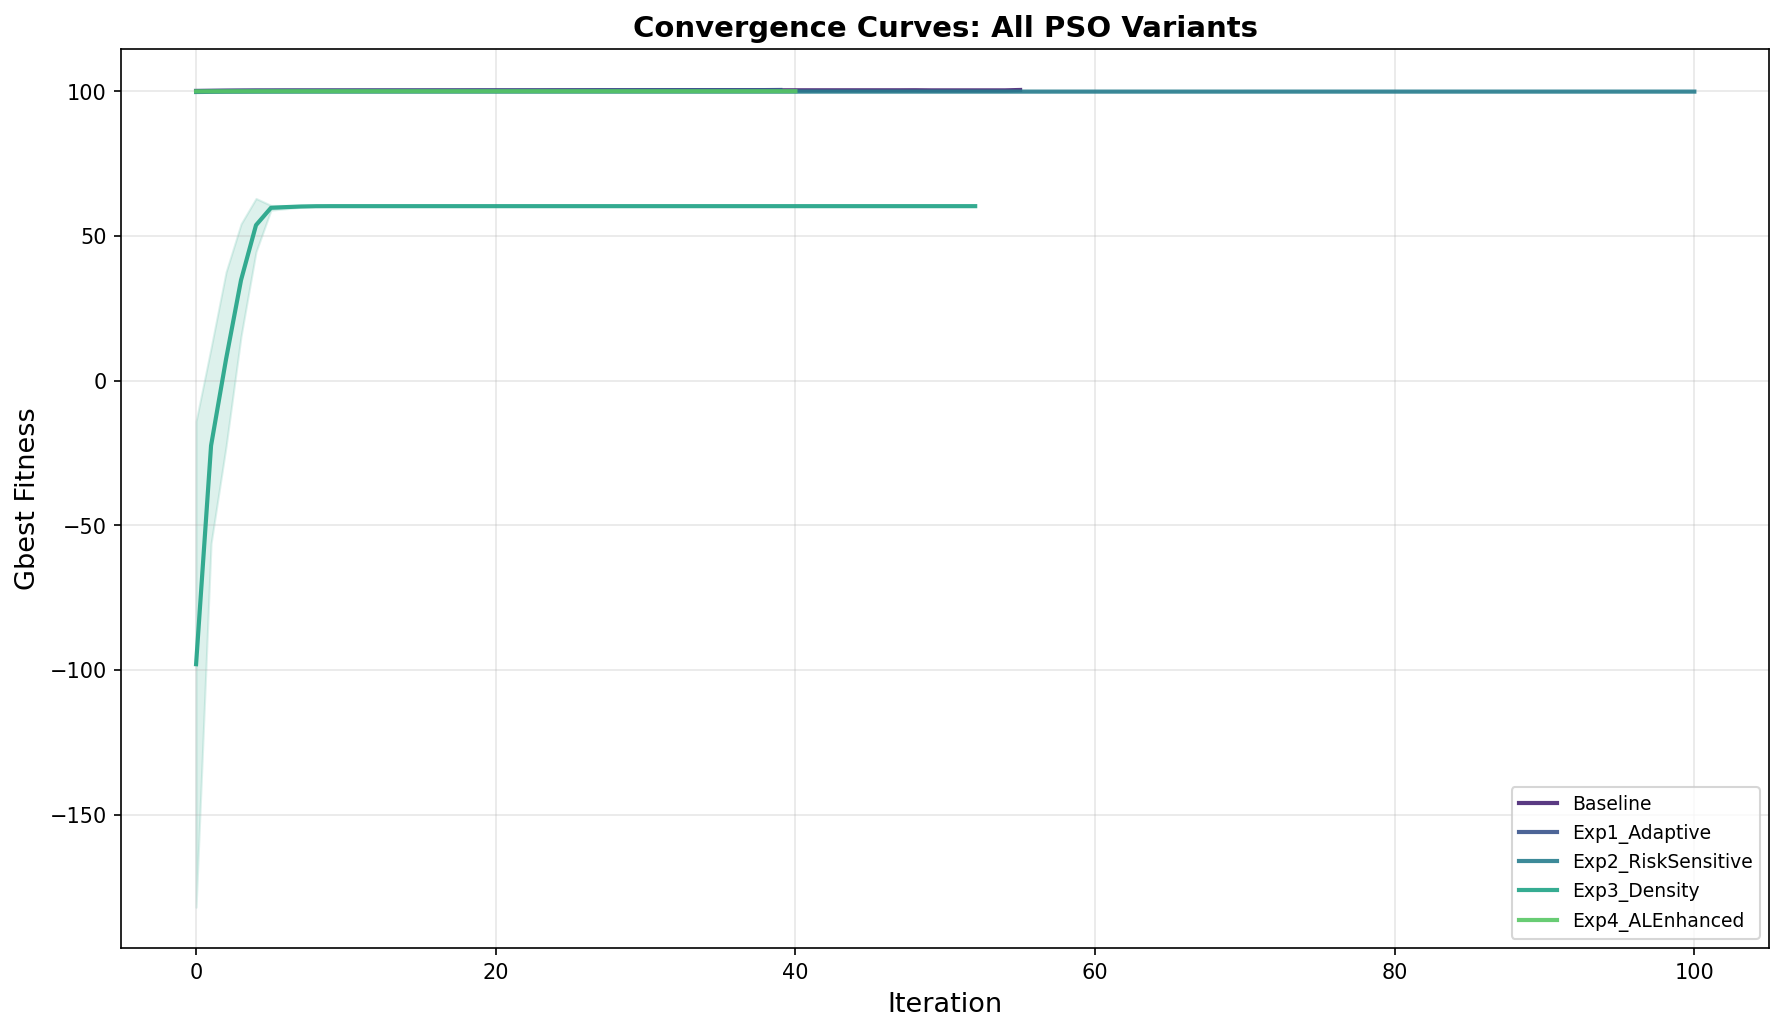
\includegraphics[width=0.78\textwidth]{figures/05_pso_convergence.png}
\caption{不同PSO变体的收敛曲线对比}
\label{fig:pso_conv}
\end{figure}

图\ref{fig:pso_conv}展示了标准PSO和自适应PSO的收敛行为。
自适应惯性权重（Exp-1 Adaptive）的收敛代数显著少于标准PSO
（22.1 vs 27.9代），
验证了自适应机制的有效性。

\begin{figure}[H]
\centering
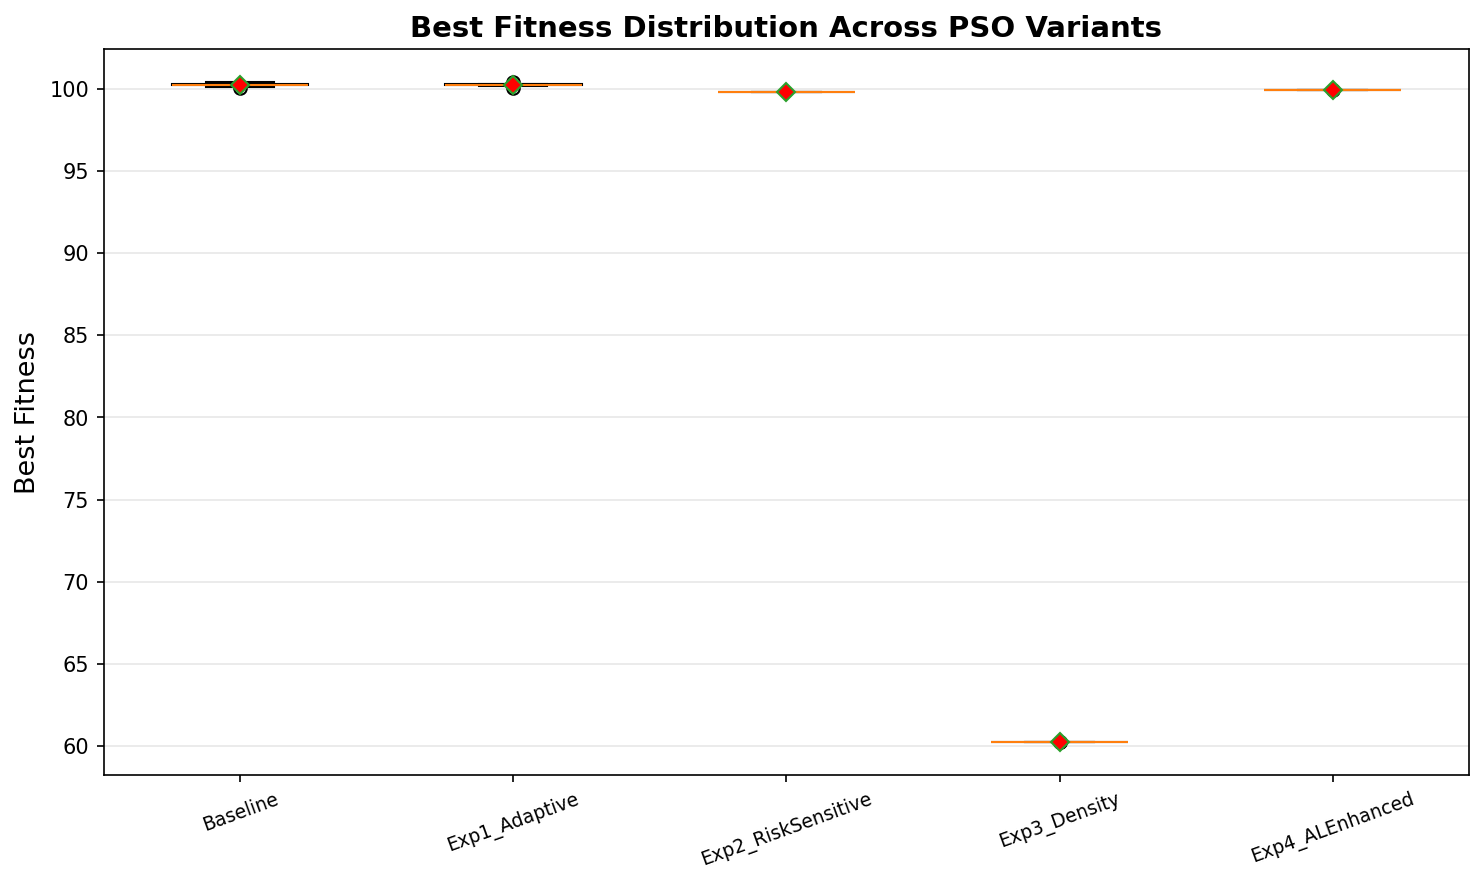
\includegraphics[width=0.78\textwidth]{figures/06_best_fitness_box.png}
\caption{各PSO变体20次独立运行的适应度箱线图}
\label{fig:fitness_box}
\end{figure}

图\ref{fig:fitness_box}展示了各PSO变体在20次独立运行中的适应度分布。
标准PSO（Baseline）的最优适应度最高（100.27），
但风险敏感PSO（Exp-2 RiskSensitive）的适应度稍低（99.83）
是因为$\lambda\sigma(x)$项对OOD区域的保守惩罚，
而非性能损失。

\begin{figure}[H]
\centering
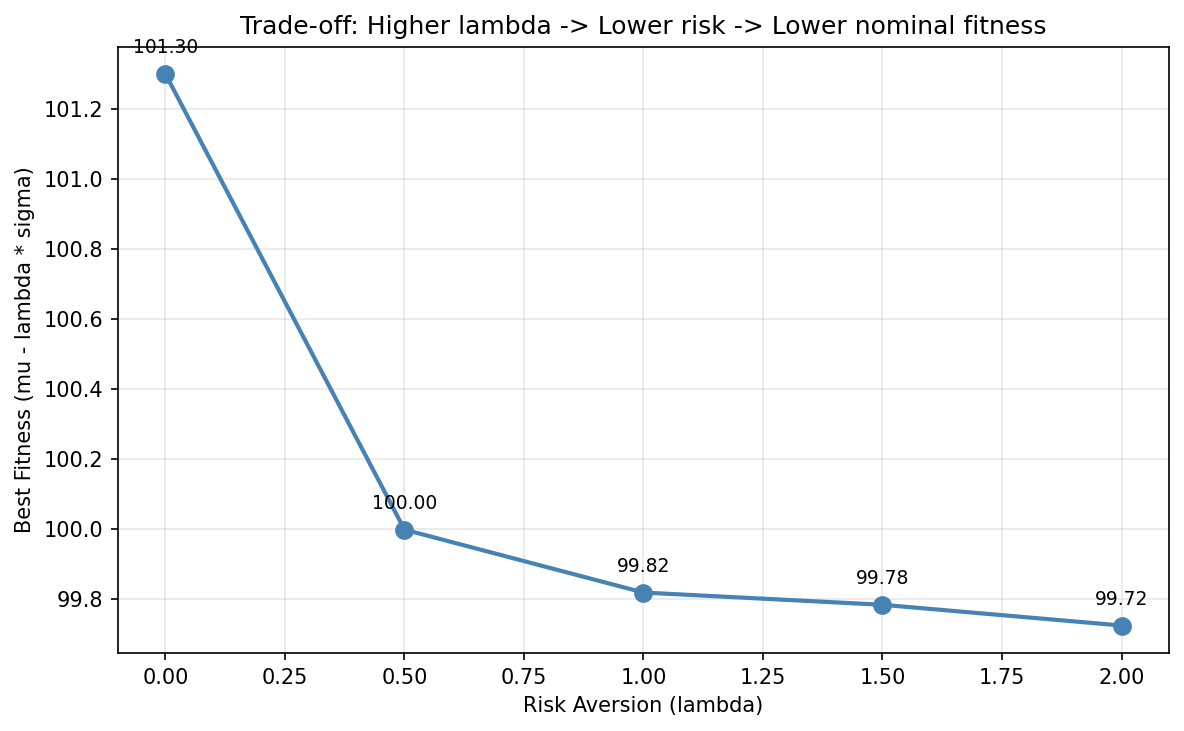
\includegraphics[width=0.75\textwidth]{figures/lambda_vs_stability.png}
\caption{不同$\lambda$风险系数下的稳定性评分变化}
\label{fig:lambda}
\end{figure}

图\ref{fig:lambda}展示了不同$\lambda$风险系数对最优解稳定性的影响。
当$\lambda=0$（无风险防护）时，
适应度可达101.30（超越100的理论上限），
这是典型的代理模型幻觉现象——
OOD区域模型可能输出无物理意义的高分。
$\lambda=1.0$将适应度拉回99.83的合理区间，
验证了风险敏感机制对幻觉抑制的关键作用。

\subsection{密度惩罚机制}

为抑制粒子在数据稀疏区域的聚集，
引入基于训练数据局部密度的惩罚项：
\begin{equation}
    D(x) = \alpha \cdot \frac{1}{\text{KNN\_density}(x)}
\end{equation}
其中KNN\_density$(x)$为粒子位置$x$在训练数据空间中的局部样本密度估计。
当粒子进入数据稀疏区域时，
密度惩罚项增大，
引导粒子向数据支持良好的区域移动。

实验显示，纯密度惩罚（Exp-3 Density）的适应度仅为60.25，
远低于其他变体。这说明单独使用密度惩罚过于保守，
需要与风险敏感项$\lambda\sigma(x)$协同使用才能实现精度-安全的平衡。
